\documentclass{extbook}
\usepackage[utf8]{inputenc}

\usepackage{mathtools}
\usepackage{listings, xcolor}
\usepackage{color}
\usepackage{geometry}
\usepackage{graphicx}
\usepackage{proof}
\usepackage{syntax}
\usepackage{hyperref}
\usepackage{tikz-qtree}

\DeclareUnicodeCharacter{03BB}{$\lambda$}
\DeclareUnicodeCharacter{03C4}{$\tau$}
\DeclareUnicodeCharacter{03B1}{$\alpha$}
\DeclareUnicodeCharacter{27F6}{$\rightarrow$}
\DeclareUnicodeCharacter{0393}{$\Gamma$}
\DeclareUnicodeCharacter{2205}{$\emptyset$}
\DeclareUnicodeCharacter{0394}{$\Delta$}


\newgeometry{
left=   1 in,
bottom= 1.5 in,
right=  1 in,
top=    1 in
}

\definecolor{bluekeywords}{rgb}{0.13,0.13,1}
\definecolor{greencomments}{rgb}{0,0.5,0}
\definecolor{turqusnumbers}{rgb}{0.17,0.57,0.69}
\definecolor{redstrings}{rgb}{0.5,0,0}

\lstdefinelanguage{FSharp}
		{morekeywords={let, new, match, with, rec, open, module, namespace, type, of, member, and, for, in, do, begin, end, fun, function, try, mutable, if, then, else,type},
    keywordstyle=\color{bluekeywords},
    sensitive=false,
    morecomment=[l][\color{greencomments}]{///},
    morecomment=[l][\color{greencomments}]{//},
    morecomment=[s][\color{greencomments}]{{(*}{*)}},
    morestring=[b]",
    stringstyle=\color{redstrings}
}

\lstdefinelanguage{Java}
		{morekeywords={for,println, public, extends, private, this, new, abstract},
    keywordstyle=\color{bluekeywords},
    sensitive=false,
    morecomment=[l][\color{greencomments}]{///},
    morecomment=[l][\color{greencomments}]{//},
    morecomment=[s][\color{greencomments}]{{(*}{*)}},
    morestring=[b]",
    stringstyle=\color{redstrings}
}

\lstdefinestyle{FSharpStyle}{
  language=FSharp,
  aboveskip=3mm,
  belowskip=6mm,
  showstringspaces=false,
  columns=flexible,
  basicstyle={\small\ttfamily},
  breaklines=true,
  breakatwhitespace=true
  tabsize=3
}

\lstdefinestyle{JavaStyle}{
language = Java,
aboveskip=3mm,
belowskip=6mm,
showstringspaces=false,
columns=flexible,
basicstyle={\small\ttfamily},
breaklines=true,
breakatwhitespace=true
tabsize=3
}

\tikzset{every tree node/.style={minimum width=2em,draw,circle},
         blank/.style={draw=none},
         edge from parent/.style=
         {draw,edge from parent path={(\tikzparentnode) -- (\tikzchildnode)}},
         level distance=1.5cm}

\definecolor{mygray}{HTML}{e1e7eb}

\title{Functional Languages Notes}
\author{Riccardo Cappi}
\date{January 2024}

\begin{document}

\maketitle

\section{Disclaimer}
These are just my notes that I used to prepare for the exam. So, probably, there will be both spelling and conceptual errors. Feel free to contact me at riccardo.cappi@studenti.unipd.it if you find any errors. This is the github repo where you can find the latex files of the notes: \url{https://github.com/riccardocappi/Computer-Science-notes}\\\\
Unfortunately the notes for this course are \textbf{incomplete} :(

\tableofcontents

\chapter{Lec 09 - Neural Networks III}

\section{Other activation functions}
Multiple layers of cascaded units makes a Neural Network able to implement complex non linear functions. The non linearity of the model is given by the activation functions. In fact, without them (linear activation) the result of the model, even if it’s very complex, would still be linear. If we used step activation functions we wouldn't be able to resort to gradient descent to optimize the weights. This is because step function is not derivable. We have to choose one or more activation functions that are derivable.
\begin{itemize}
    \item \textbf{Sigmoid:}
    \[\sigma(y) = \frac{1}{1 + e^{-y}}\]

    \item \textbf{ReLu:}
    \[r(y) = max(0, y)\]
\end{itemize}
\section{Multi-layer Neural Networks: Keywords}
Let's define the most important keywords for Multi-layer Neural Networks:
\begin{itemize}
    \item $d$ \textbf{input units}: $d$ input data size $\textbf{x} \equiv (x_{1},...,x_{d})$, $d + 1$ when including the bias in the weight vector $\textbf{x}^{'} \equiv (x_{0}, x_{1},...,x_{d})$

    \item $n_{H}$ \textbf{hidden units} (with output $\textbf{y} \equiv (y_{1},...,y_{n_{H}})$)

    \item $c$ \textbf{output units}: $\textbf{z} \equiv (z_{1},...,z_{c})$. The number of desired output is $\textbf{t} \equiv (t_{1},...,t_{c})$

    \item $w_{ji}$ weight from the $i$-th input unit to the $j$-th hidden unit ($w_{j}$ is the weight vector of the $j$-th hidden unit)

    \item $w_{kj}$ weight from the $j$-th hidden unit to the $k$-th output unit ($w_{k}$ is the weight vector of the $k$-th output unit)
\end{itemize}
\section{Learning algorithm}
Let's consider, for example, a Neural Network with just one hidden layer and \textbf{sigmoid activation functions}. The basic idea of the learning algorithm consists in two phases:
\begin{itemize}
    \item \textbf{Forward phase:} for each example in the training set, present it to the network and compute the output.
    \item \textbf{Backward phase:} Back-propagate the committed error and update the weights of the hidden units accordingly. 
\end{itemize}
This algorithm is called \textbf{Backpropagation}\newline\newline
As we said before, this algorithm is based on gradient descent, so we need to minimize an error function $E[\textbf{w}]$ that can be defined as follows:
\[E[\textbf{w}] = \frac{1}{2cN}\sum_{s=1}^{N}\sum_{k=1}^{c}(t_{k}^{(s)} - z_{k}^{(s)})^{2}\]
In order to implement Backpropagation, we need to first compute the gradient for the weights of both output and hidden units.
\begin{itemize}
    \item \textbf{Gradient of the weights of an output unit:}
    \[\frac{\partial E}{\partial w_{\hat{k}\hat{j}}} = - \frac{1}{cN}\sum_{s=1}^{N}(t_{\hat{k}}^{(s)} - z_{\hat{k}}^{(s)} )z_{\hat{k}}(1 - z_{\hat{k}})y_{\hat{j}}^{(s)}\]
    where $y_{\hat{j}}^{(s)}$ is the output of the $\hat{j}$-th hidden unit.
    
    \item \textbf{Gradient of the weights of a hidden unit:}
    \[\frac{\partial E}{\partial w_{\hat{j}\hat{i}}} = - \frac{1}{cN}\sum_{s=1}^{N}y_{\hat{j}}^{(s)}(1 - y_{\hat{j}}^{(s)})x_{\hat{i}}^{(s)}\sum_{k=1}^{c}(t_{\hat{k}}^{(s)} - z_{\hat{k}}^{(s)} )z_{\hat{k}}(1 - z_{\hat{k}})w_{k\hat{j}}\]
\end{itemize}
Note that, for simplicity, we are considering a Neural Network with just one hidden layer, but the derivation can be extended for more than one hidden layer.
\subsection{Back-propagation algorithm}
Back-propagation is an algorithm that aims to update the weights of a Neural Network in order to minimize the error between the predicted output and the true output. The algorithm works by propagating the error back through the network, starting with the output layer and moving backwards through the hidden layers, adjusting the weights at each layer to reduce the error. It can be implemented in different ways:
\begin{itemize}
    \item \textbf{Batch gradient descent:} It \textbf{cumulates} gradients over all the training examples and then updates the weights.
    \item \textbf{Stochastic gradient descent:} For each example in $S$, it computes the gradients and update the weights.
    \item \textbf{Mini-batch gradient descent:} It updates the weights considering a subset of examples $Q \subseteq S$. 
\end{itemize}
This process is typically repeated many times until the error is sufficiently small or the maximum number of iterations is reached. Let's define the algorithm according to the derivations seen before:\newline\newline
\textbf{Back-propagation (stochastic)}
\begin{enumerate}
    \item Initialize all weights with small random values (e.g. between -0.5 and +0.5)
    \item Until the termination condition is satisfied:
    \begin{enumerate}
        \item For each $(\textbf{x},\textbf{t}) \in S$:
        \begin{enumerate}
            \item Present $\textbf{x}$ to the net and compute the vectors $\textbf{y}$ and $\textbf{z}$
            \item For each output unit $k$:
            \[\delta_{k} = z_{k}(1 - z_{k})(t_{k} - z_{k})\]
            \[\Delta w_{kj} = \delta_{k}y_{j}\]

            \item For each hidden unit $j$:
            \[\delta_{j} = y_{j}(1 - y_{j})\sum_{k=1}^{c}w_{kj}\delta_{k}\]
            \[\Delta w_{ji} = \delta_{j}x_{i}\]

            \item Update all weights:
            \[w_{sq} \leftarrow w_{sq} + \eta \Delta w_{sq}\]
        \end{enumerate}
    \end{enumerate}
\end{enumerate}
Note that this algorithm works only for a network with one hidden layer, but can be easily extended. In fact, the algorithm computes the error term $\delta$ for each unit of each layer, and then it multiplies this error term for the input of the unit.

\section{Computational power of neural networks}
\textbf{Theorem (Pinkus, 1996) simplified}:\newline
Given a feed-forward NN with just one hiddel layer, any continuous function $f:\mathbb{R}^{n} \rightarrow \mathbb{R}$ and an arbitrarily small $\epsilon > 0$, then, for a large class of activation functions, there always exists an integer $M$ such that the function $g: \mathbb{R}^{n} \rightarrow \mathbb{R}$ computed by the net using at least $M$ hidden units approximates the function $f$ with tolerance $\epsilon$, that is:
\[max_{x \in \Omega}|f(\textbf{x}) - g(\textbf{x})| < \epsilon\]
Note that the theorem attests the existence of a NN with $M$ hidden units that approximates the target function with the desired tolerance, but it says nothing about how $M$ can be computed.

\section{Fine tuning neural networks}
The choice of the net typology determines the hypothesis space used. With three-layers architecture (input, hidden, output), the number of hidden units detrmines the complexity of the hypothesis space. As we said for the Perceptron, the choice of the learning rate $\eta$ can be crucial for the convergence.
\subsection{Avoiding local minima}
The local minima problem in neural networks refers to the scenario where a neural network gets stuck in a sub-optimal solution during the training process. Instead of reaching the global minimum, which is the best possible solution, the network settles for a local minimum, that may not be the best fit for the data. This can happen because the loss function used can have multiple local minima, and the optimization algorithm may only find one of them. In order to avoid this problem, we can use different techniques:
\begin{itemize}
    \item Adding a term to the weight update rule (called \textbf{momentum}). Basically, a contribution deriving from the previous step is added, imposing a kind of inertia on the system.

    \item Using \textbf{stochastic training} (randomizing on the examples) instead of batch training can facilitate to avoid local minima.

    \item \textbf{Training multiple NNs} on the same data with different initialization and combining the outputs.
\end{itemize}

\subsection{Over-fitting}
With neural networks, usually, the error on the validation set increases as the number of weight updates increases. This is because, at the beginning, with small absolute values of the weights (similar each other), the decision surfaces are \textit{smoother}. When the absolute values of the weights increase , the complexity of the decision surfaces increases and with it the possibility to suffer over-fitting. \newline\newline
A possible solution can be to use an additional term in the error function to minimize based on the norm of the weights (regularization) $E + ||w||^{2}$.

\section{Hidden layer representation}
An important feature of multi-layer NNs is that they can find useful representations of input data (alternative to the input representation). Specifically, the output of the hidden units is an effective new input representation for the next layers. This feature can be used to define a particular type of NNs called Auto-encoders.


\chapter{Lec 10 - Generalized Linear Models and SVM I}
\section{Linear Models}
Linear models are one of the most important types of models in machine learning. A linear model is of the form:
\[f_{\textbf{w},b}(\textbf{x}) = \sum_{i=1}^{m} w_{i}x_{i} + b = \textbf{w} \cdot \textbf{x} + b\]
Which can also be written as
\[f_{\textbf{w},b}(\textbf{x}) = \sum_{i=0}^{m} w_{i}x_{i}= \textbf{w} \cdot \textbf{x}\]
where $x_{0} = 1$.
\begin{itemize}
    \item For \textbf{classification}, the sign of the result is returned, that is:
    \[h(\textbf{x}) = sign(f_{\textbf{w}}) \in \{-1, +1\}\]

    \item For \textbf{regression}, the \textit{original} function can be taken, that is:
    \[h(\textbf{x}) = f_{\textbf{w}} \in \mathbb{R}\]
\end{itemize}
\subsection{Linear Regression}
Given a training set $S = \{(\textbf{x}_{1}, y_{1}), ..., (\textbf{x}_{n}, y_{n})\}$, in linear regression we look for a hypothesis $h_{\textbf{w}}$ which minimizes the mean squared error on the training set, that is:
\[argmin_{\textbf{w}} \frac{1}{n}\sum_{i=0}^{n}(h_{\textbf{w}}(\textbf{x}_{i}) - y_{i})^{2}\]
We can formalize it in matrices terms:
\[E(\textbf{w}) = \frac{1}{n}\sum_{i=0}^{n}(h_{\textbf{w}}(\textbf{x}_{i}) - y_{i})^{2}\]
\[= \frac{1}{n}\sum_{i=0}^{n}(\textbf{w} \cdot \textbf{x}_{i} - y_{i})^{2}\]
\[= \frac{1}{n}||\textbf{Xw} - \textbf{y}||\]
where:
\begin{itemize}
    \item $\textbf{X}$ is a matrix of size $n \times d$
    \item $\textbf{w}$ is a vector of size $d \times 1$
    \item $\textbf{y}$ is a vector of size $n \times 1$
\end{itemize}
$d$ is the dimension of the feature space (including the bias term). Basically, we want that $\textbf{Xw} \approx \textbf{y}$.\newline\newline
Since $||\vec{z}||^{2} = \sum_{i}z_{i}^{2}$, the optimization problem can be defined as follows:
\[min_{\textbf{w}}E(\textbf{w}) \equiv \frac{1}{n}||\textbf{Xw} - \textbf{y}||^{2}\]
We want to find the vector $\textbf{w}$ that minimizes $E$. Basically, we want to find the points $\textbf{w}$ where the gradient vanishes (equals to 0), that is:
\[\nabla E(\textbf{w}) = \frac{2}{n}\textbf{X}^{T} (\textbf{Xw} - \textbf{y}) = 0\]
\[\textbf{X}^{T}\textbf{Xw} = \textbf{X}^{T}\textbf{y}\]
By multiplying the quantity $(\textbf{X}^{T}\textbf{X})^{-1}$ both on the left and on the right of the equation, it becomes:
\[(\textbf{X}^{T}\textbf{X})^{-1}(\textbf{X}^{T}\textbf{X})\textbf{w} = (\textbf{X}^{T}\textbf{X})^{-1}\textbf{X}^{T}\textbf{y}\]
Since $(\textbf{X}^{T}\textbf{X})^{-1}(\textbf{X}^{T}\textbf{X})$ is the identity matrix, the final equation is:
\[\textbf{w} = (\textbf{X}^{T}\textbf{X})^{-1}\textbf{X}^{T}\textbf{y}\]
This is a \textbf{closed form solution}. It means that with just one computation we are able to find the solution, it's not am iterative process. However, computing the inverse of a matrix can be very computational inefficient.

\subsection{Non-linear mapping}
The goal of non-linear mapping is to apply a transformation to non-linearly separable points in order to map them in a new feature space that is linearly separable. Then, a linear model (hyperplane) in the transformed space will correspond to a non-linear decision surface in the original space (Generalized Linear Models).

\section{Linear separability}
Consider the hypothesis space of hyperplanes. Given a set of linearly separable points, we have different hyperplanes that separates them. Intuitively, the widest possible margin (or \textbf{optimal}) hyperplane is the best one, because is the one that generalizes better, but how can we compute to which $\textbf{w}$, $b$ the best hyperplane corresponds.
\subsection{Margin of a hyperplane}
The margin of a hyperplane is the distance between the hyperplane and the closest data points of each class. \newline\newline
Let's consider the \textbf{binary classification} problem. Given the hyperplane $\textbf{w} \cdot \textbf{x} + b = 0$ (\textbf{optimal hyperplane}), the \textit{"distance"} of a point $\textbf{x}$ from the hyperplane can be expressed by the algebraic measure $g(\textbf{x}) = \textbf{w}^{T} \cdot \textbf{x} + b$. We can write $\textbf{x}$ as follows:
\[\textbf{x} = \textbf{x}_{p} + r\frac{\textbf{w}}{||\textbf{w}||}\]
where:
\begin{itemize}
    \item $||\textbf{w}||$ is the norm of $\textbf{w}$
    \item $\textbf{x}_{p}$ is the normal projection of $\textbf{x}$ onto the hyperplane.
    \item $r$ is the desired algebraic distance ($r > 0$ if $\textbf{x}$ is on the positive side of the hyperplane, otherwise $r < 0$).
\end{itemize}
Note that $g(\textbf{x}_{p}) = 0$ because $\textbf{x}_{p}$ is on the hyperplane. Furthermore, since we are considering the optimal hyperplane, the absolute distance between this hyperplane and any nearest positive example is the same as the absolute distance between any negative example. So, we can \textit{normalize} the value of $g$ such that $g(\textbf{x}) = 1$ if $\textbf{x}$ is in the positive margin hyperplane and $g(\textbf{x}) = -1$ if $\textbf{x}$ is in the negative margin hyperplane.\newline\newline
Take $\textbf{x}_{k}$ in the positive margin hyperplane, it follows that
\[g(\textbf{x}_{k}) = \textbf{w}^{T}\textbf{x}_{k} + b\]
Since $\textbf{x}_{k} = \textbf{x}_{p} + r\frac{\textbf{w}}{||\textbf{w}||}$:
\[= \textbf{w}^{T}\left(\textbf{x}_{p} + r\frac{\textbf{w}}{||\textbf{w}||}\right) + b\]
\[= \textbf{w}^{T}\textbf{x}_{p} + b + r\frac{\textbf{w}^{T}\textbf{w}}{||\textbf{w}||}\]
Since $\textbf{w}^{T}\textbf{w} = ||\textbf{w}||^{2}$:
\[= \textbf{w}^{T}\textbf{x}_{p} + b + r||\textbf{w}||\]
The term $\textbf{w}^{T}\textbf{x}_{p} + b = 0$ because, as we said before, $g(\textbf{x}_{p}) = 0$. This implies that:
\[g(\textbf{x}_{k}) = r||\textbf{w}|| = +1\]
This is true only if
\[r = \frac{1}{||\textbf{w}||}\]
Then, the margin $\rho$ is defined as follows:
\[\rho = 2r = \frac{2}{||\textbf{w}||}\]
\section{Support Vector Machines (SVM)}
Support Vector Machines (SVMs) are a set of supervised learning methods used for classification and regression tasks. The idea behind SVMs is to find the best hyperplane that separates the training data. This hyperplane is chosen in such a way that it maximizes the margin.
\subsection{Separable case: Quadratic optimization}
If we have $n$ linearly separable examples $\{(\textbf{x}_{i}, y_{i})\}$ (binary classification), it is possible to find the optimal hyperplane $h(\textbf{x}) = sign(\textbf{w} \cdot \textbf{x} + b)$ by solving the following \textbf{constrained} quadratic optimization problem:
\[min_{\textbf{w},b}\frac{1}{2}||\textbf{w}||^{2}\]
\[subject \,\, to: \,\, \forall i \in \{1,...,n\}: y_{i}(\textbf{w} \cdot \textbf{x}_{i} + b) \geq 1\]
Since the margin is defined as $\rho = \frac{2}{||\textbf{w}||}$ and we want to maximize it, we need to minimize $||\textbf{w}||$. This minimization problem is subject to the constraint that each point in the training set must be on the \textit{correct} side of the hyperplane, which means that for each point, the following inequality must hold: $\forall i \in \{1,...,n\}: y_{i}(\textbf{w} \cdot \textbf{x}_{i} + b) \geq 1$. This constraint is given by the fact that:
\begin{itemize}
    \item $\textbf{w} \cdot \textbf{x}_{i} + b \geq 1$ if $y_{i} = +1$
    \item $\textbf{w} \cdot \textbf{x}_{i} + b \leq 1$ if $y_{i} = -1$
\end{itemize}
This is a \textbf{convex} constrained quadratic problem, and for this reason it guarantees a unique solution.\newline\newline
With a large number of features it can be computationally inefficient to solve this problem, so we can use its \textbf{dual formulation}
\subsection{Dual formulation}
In the dual problem, Lagrange multipliers $\alpha_{i} \geq 0$ are associated with every constraint in the primal problem (one for each example).
\[max_{\alpha} \sum_{i=1}^{n}\alpha_{i} - \frac{1}{2}\sum_{i,j=1}^{n}y_{i}y_{j}\alpha_{i}\alpha_{j}(\textbf{x}_{i} \cdot \textbf{x}_{j})\]
\[subject \,\, to: \,\, \forall i \in \{1,...,n\}: \,\, \alpha_{i} \geq 0 \,\, and \,\, \sum_{i=1}^{n}y_{i}\alpha_{i} = 0\]
At the solution, most of the $\alpha_{i}$'s are zeros. Those examples associated with non zero multipliers are called \textbf{support vectors}.

\subsection{SVM solution}
The primal solution turns out to be:
\[\textbf{w} = \sum_{i=1}^{n}y_{i}\alpha_{i}\textbf{x}_{i}\]
\[b = y_{k} - \textbf{w} \cdot \textbf{x}_{k}\,\, \forall \textbf{x}_{k}\,\,s.t\,\, \alpha_{k} > 0\]
Hence:
\[h(\textbf{x}) = sign(\textbf{w} \cdot \textbf{x} + b) = sign\left(\sum_{i = 1 \in support \,\, vector}^{n}y_{i}\alpha_{i}(\textbf{x}_{i} \cdot \textbf{x}) + b\right)\]
The decision function only depends on dot products between the point and othe points in the training set (the support vectors).

\chapter{Lec 11 - NP-Hardness}

\section{Tractable vs Intractable problems}
Problems for which a polynomial algorithm exists are called \textbf{tractable}. If no such algorithm exists, the problem is called \textbf{intractable}.\newline\newline
\textbf{Examples:}
\begin{enumerate}
    \item \textbf{Eulerian circuit problem:} Given an undirected graph, an Eulerian circuit is a cycle that traverses all the edges only once. This problem can be solved in linear time. Note that in an Euler circuit you might pass through a vertex more than once.

    \item \textbf{Hamiltonian circuit problem:} Given an undirected graph, an Hamiltonian circuit is a cycle that traverses all the vertices only once. To date, no one knows a polynomial algorithm to solve it. Note that in a Hamiltonian circuit you may not pass through all edges.

    \item \textbf{Minimum spanning tree:}

    \item \textbf{Traveling Salesperson Problem (TSP):} Given a complete, undirected graph and a function $w: E \rightarrow \mathbb{R}$, output a \textbf{tour} (i.e. a cycle that visits every vertex exactly once) of minimum cost
    \[T \subseteq E \quad \text{minimizing }\sum_{e \in T}w(e)\]
    To date, no one knows a polynomial algorithm to solve it.
\end{enumerate}
A much easier task can be the following: Given a graph and a list of vertices $C$, \textbf{check} if $C$ is an Hamiltonian circuit.\newline\newline
Problems that are \textit{easy} to solve belong to the \textbf{complexity class} \textbf{P} (\textit{polynomial time}), 1), 3) $\in$ \textbf{P}. Problems that are \textit{easy} to verify belong to the complexity class \textbf{NP} (\textit{Non-deterministic polynomial}), 1), 2) ,3) ,4) $\in$ \textbf{NP}.

\section{NP-Hard}
\textbf{Decision Problems:}\newline
To simplify the study of the complexity of problems, we limit our attention to problems with a boolean answer (YES, NO), that is, decision problems.\newline\newline
Let's define \textbf{P} and \textbf{NP} classes in a more formal way:
\begin{itemize}
    \item \textbf{P} is the set of decision problems that can be solved in polynomial time.

    \item \textbf{NP} is the set of decision problems with the following property: if the answer is YES, then there is a proof of this fact that can be checked in polynomial time.

    \item \textbf{NP-Hard:} A computational problem is \textbf{NP-Hard} if a polynomial-time algorithm that solves it would imply a polynomial-time algorithm that solves every problem in \textbf{NP}.\newline\newline
    A problem is \textbf{NP-Complete} if it is both in \textbf{NP} and \textbf{NP-Hard}. Basically, these problems are the hardest in \textbf{NP}. 
\end{itemize}
\begin{figure}[h]
    \centering
    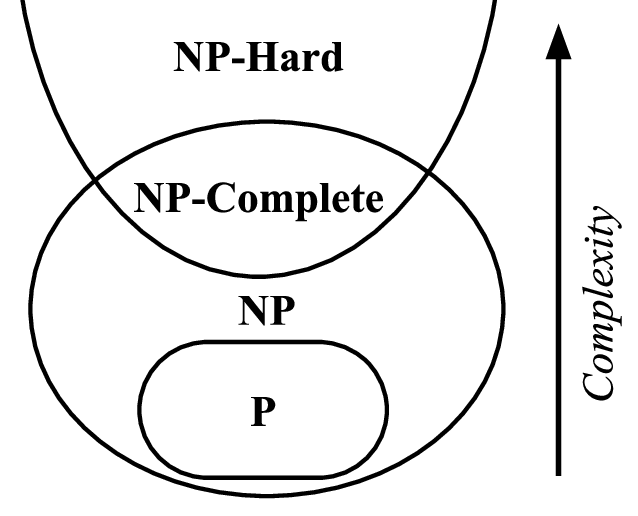
\includegraphics[scale=0.4]{images/P-NP.png}
    \caption{What we think the computation classes look like}
    \label{fig:P-NP-Np-Hard}
\end{figure}
One of the main open questions in computer science is whether \textbf{P=NP}.\newline\newline
Studying NP-Hardness is important because if a problem is \textbf{NP-Hard} is a strong evidence that it is intractable. It suggests you to use a different approach, such as identify tractable special-cases, or use \textbf{approximation algorithms}.

\section{Cook-Levin Theorem}
\textit{In computational complexity theory, the Cook–Levin theorem, also known as Cook's theorem, states that the Boolean satisfiability problem is \textbf{NP-complete}.}\footnote{Wikipedia definition}\newline\newline
SAT: formula satisfiability:
\begin{itemize}
    \item input: A boolean formula like the following: $(b \land \neg c) \lor (\neg a \land b)$

    \item output: It is possible to assign boolean values to the variables $a, b, c, ...$ such that the entire formula evaluates to TRUE?
\end{itemize}
determining the satisfiability of a formula in conjunctive normal form (CNF) where each clause is limited to at most three literals is \textbf{NP-complete} also; this problem is called \textbf{3-SAT}.\newline\newline
\textbf{Example of 3-CNF formula:}
\[(a \lor b \lor c) \land (b \lor \neg c \lor \neg d) \land (\neg a \lor c \lor d)\]
%Check if the theorem was defined on 3SAT???
How can we show that a problem is \textbf{NP-Hard}?

\section{Reductions}

To prove that a problem $P$ is \textbf{NP-Hard} we use \textbf{reduction}. We want to prove that every problem in \textbf{NP} reduces to problem $P$.\newline\newline
Reducing problem $A$ to problem $B$ means describing an algorithm to solve $A$ under the assumption that an algorithm for $B$ exists.
\begin{center}
    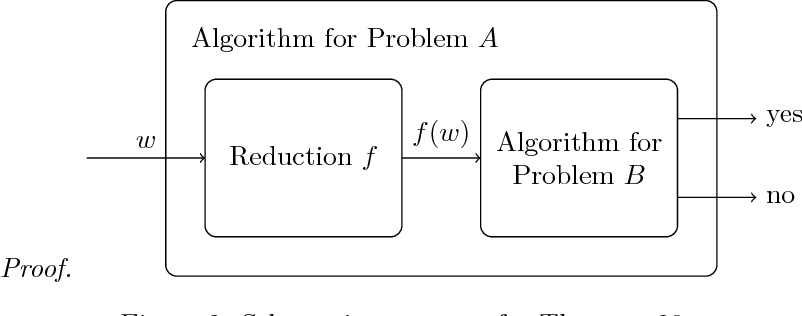
\includegraphics[scale=0.4]{images/Reduction.png}
\end{center}
$A < B$ means \textit{A reduces to B} where $B$ is the hardest problem ($A$ is as hard as $B$).


\chapter{Lec 12 - Preprocessing}

\section{Supervised learning pipeline}
The supervised learning pipeline can be summarized as follows:
\begin{enumerate}
    \item Analysis of the problem (Classification, Regression, ...)

    \item Collection, analysis and cleaning data

    \item Pre-processing and managing missing values

    \item Study of correlation between variables 

    \item Feature selection/weighting/learning

    \item Choice of the predictor and model selection

    \item Test
\end{enumerate}
Some of the most common objects that we can find in machine learning are:
\begin{itemize}
    \item \textbf{Vectors} (Set of values)
    \item \textbf{Strings}
    \item \textbf{Sets and Bags}: for example, the set of terms in a document or their frequency
    \item \textbf{Tensors}: for example, images and video
    \item \textbf{Trees and graphs}
\end{itemize}
The easiest way to represent these objects is to map them in a vectorial representation.\newline\newline
Features values can be divided in two classes: \textbf{Categorical} and \textbf{Quantitative}:
\begin{itemize}
    \item Categorical or symbolic features
    \begin{itemize}
        \item Nominals: They are used for naming or labeling variables, without any quantitative value. There is usually no intrinsic ordering to nominal data.

        \item Ordinals: Is a type of categorical data with an order.
    \end{itemize}

    \item Quantitative and numeric features:
    \begin{itemize}
        \item Intervals (Enumerables)
        \item Ration (Real values)
    \end{itemize}
\end{itemize}
Let's see how to encode categorical and quantitative variables into a vector.

\section{Encoding categorical or symbolic variables}
One of the most common method to encode a categorical variable into a vector is the \textbf{OneHot Encoding}. This technique allows you to represents categorical variables in a vector with as many components as the number of possible values for the variable.\newline\newline
For example, let's say that we want to encode a variable corresponding to the brand of a car. The possible values that an instance can take are: \textit{(Fiat, Toyota, Ford)}. The OneHot encoding of an instance having \textit{Toyota} as brand value could be the following: $[0, 1, 0]$. Basically, it's a vector where we set to one the component corresponding to the value of the instance.

\section{Encoding of continuous variables}
In this case, it is more difficult to find a good mapping. Therefore, the features are typically transformed to obtain values \textit{comparable} with other features.\newline\newline
Given a matrix of instances (training set), for each feature $j$, let $\hat{x}_{j} = \frac{1}{n}\sum_{i=1}^{n}x_{ij}$ be the average value of the current feature and let $\sigma_{j} = \sqrt{\frac{1}{n}\sum_{i=1}^{n}(x_{ij} - \hat{x}_{j})^{2}}$ be the standard deviation of $j$. We can apply the following transformations:
\begin{itemize}
    \item Centering: $c(x_{ij}) = x_{ij} - \hat{x}_{j}$. For each value $x_{ij}$ we compute $c(x_{ij})$ which is equal to the difference between the value and the average of the corresponding feature.

    \item Standardization: $s(x_{ij}) = \frac{c(x_{ij})}{\sigma_{j}}$. We want the \textit{columns} (features) of the matrix to have mean equals to 0 and variance equals to 1.

    \item Scaling to a range: $h(x_{ij}) = \frac{x_{ij} - x_{min j}}{x_{max j} - x_{min j}}$. Each value is scaled in a range between 0 and 1.

    \item Normalization: $g(\textbf{x}) = \frac{\textbf{x}}{||\textbf{x}||}$. In this case, we don't work over features but we want to normalize the instances (rows).
\end{itemize}
The python module \textit{sklearn} provides several methods to perform this kind of pre-processing.

\subsection{K-Nearest Neighbors}
K-Nearest Neighbors is a simple classification algorithm where a test example is classified with the majority class of its k-neighbors in the training set.\newline\newline
When the instances are \textbf{normalized} we can define the squared distance between them in terms of dot-product:
\[||\textbf{x} - \textbf{z}||^{2}\]
\[= ||\textbf{x}||^{2} + ||\textbf{z}||^{2} - 2\langle \textbf{x}, \textbf{z}  \rangle\]
Since the norm of the instances is equal to 1, it follows that:
\[= 2 - 2\langle \textbf{x}, \textbf{z}  \rangle\]
So, with normalized data, the distance between two instances is inversely proportional to their dot-product.

\section{Feature selection and feature extraction}
Feature \textbf{selection} is the reduction of the dimensionality of the features obtained by removing irrelevant or redundant features. The interpretability of the model is maintained.\newline\newline
Feature \textbf{extraction} is the reduction of the dimensionality of the features obtained by combining the original features (e.g. PCA). Generally, the interpretability of the model is lost.

\subsection{Feature selection}
The top reasons to use feature selection are:
\begin{itemize}
    \item It enables the machine learning algorithm to train faster

    \item It reduces the complexity of a model and makes it easier to interpret.

    \item It improves the accuracy of a model if the right subset is chosen.

    \item It reduces over-fitting.
\end{itemize}
Feature selection methods can be divided in 3 classes:
\begin{itemize}
    \item \textbf{Filter methods:} They perform feature selection before applying the predictor. They use an efficient scoring function (e.g. Mutual information, Chi squared, Information gain) that determines the usefulness of a given set of features.

    \item \textbf{Wrapped methods:} The predictor is evaluated on a hold-out sample using subset of different features. Then, the subset with highest score is chosen.

    \item \textbf{Embedded methods:} The selection of features occurs in conjunction with the training of the model, for example, by modifying the objective function to be optimized. 
\end{itemize}

\subsection{Feature extraction (PCA)}
\textbf{Principal Component Analysis (PCA)} converts a set of instances with possibly related features into corresponding values on another set of linearly unrelated features (principal components).\newline\newline
\textbf{Neural Networks} can also be seen as a particular way to perform feature extraction on their hidden layers. In fact, the output values of one of the hidden layers can be considered as a new representation of the original data.


\chapter{Lec 13 - Resolution for First Order Logic}

\section{Resolution}
The last of our three families of logical systems is based on \textbf{resolution}. In resolution for first order logic two clauses, which are assumed to be standardized apart so
that they share no variables, can be resolved if they contain complementary literals. Propositional literals are complementary if one is the negation of the other; first-order literals are complementary if one unifies with the negation of the other. Thus, we have
\begin{center}
    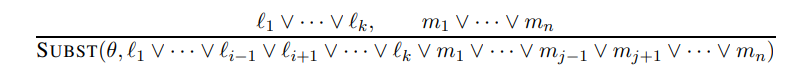
\includegraphics[]{images/resolution-fol.png}
\end{center}
where $UNIFY(l_i,\neg{m_j} ) = \theta$. For example, we can resolve the two clauses
\[[Animal(F(x)) \lor Loves(G(x), x)]\,\, \text{and} \,\,[\neg Loves(u, v) \lor \neg Kills(u, v)]\]
by eliminating the complementary literals $Loves(G(x), x)$ and $\neg Loves(u, v)$, with unifier $\theta = \{u/G(x), v/x\}$, to produce the \textbf{resolvent} clause
\[[Animal(F(x)) \lor \neg Kills(G(x), x)] .
\]
Then, the resolution steps can be applied to $CNF(KB \land \neg \alpha)$ as we did for propositional logic.

\section{Conversion to CNF}
As in the propositional case, first-order resolution requires that sentences be in \textbf{conjunctive
normal form} (CNF), that is, a conjunction of clauses, where each clause is a disjunction of literals. Literals can contain variables, which are assumed to be universally quantified. Every sentence of first-order logic can be converted into an inferentially equivalent CNF
sentence.\\\\
We illustrate the procedure by translating the sentence “Everyone who loves all animals is loved by someone,” or
\[\forall x \, [\forall y \, Animal(y) \Rightarrow Loves(x, y)] \Rightarrow [\exists y \, Loves(y, x)].\]
The steps are as follows:
\begin{itemize}
    \item \textbf{Eliminate implications:}
    \[\forall x \, [\neg \forall y \, \neg Animal(y) \lor Loves(x, y)] \lor [\exists y \, Loves(y, x)] .\]

    \item \textbf{Move} $\neg$ \textbf{inwards}: In addition to the usual rules for negated connectives, we need rules for negated quantifiers. Thus, we have
    \[\begin{split}
        & \neg \forall x \, p \,\, \text{becomes} \,\, \exists x \, \neg p\\
        & \neg \exists x \, p \,\, \text{becomes} \,\, \forall x \, \neg p .
    \end{split}\]
    Our sentence goes through the following transformations:
    \[\begin{split}
        & \forall x \, [\exists y \, \neg(\neg Animal(y) \lor Loves(x, y))] \lor [\exists y \, Loves(y, x)].\\
        & \forall x \,[\exists y \, \neg \neg Animal(y) \land \neg Loves(x, y)] \lor [\exists y \, Loves(y, x)].\\
        & \forall x \,[\exists y \, Animal(y) \land \neg Loves(x, y)] \lor [\exists y \, Loves(y, x)]
    \end{split}
    \]

    \item \textbf{Standardize variables}: each quantifier should use a different one:
    \[\forall x \,[\exists y \, Animal(y) \land \neg Loves(x, y)] \lor [\exists z \, Loves(z, x)] .\]

    \item \textbf{Skolemize:} \textbf{Skolemization} is the process of removing existential quantifiers by elimination. In the simple case, it is just like the Existential Instantiation rule seen previously: translate $\exists x \, P(x)$ into $P(A)$, where $A$ is a new constant. However, we can’t apply Existential Instantiation to our sentence above. If we blindly apply the rule to the two matching parts we get
    \[\forall x \, [Animal(A) \land \neg Loves(x, A)] \lor Loves(B,x),\]
    which has the wrong meaning entirely: it says that everyone either fails to love a particular animal $A$ or is loved by some particular entity $B$. Thus, we want the Skolem entities to depend on $x$ and $z$:
    \[\forall x \, [Animal(F(x)) \land \neg Loves(x, F(x))] \lor Loves(G(z), x) .\]
    Here $F$ and $G$ are \textbf{Skolem functions}.  The general rule is that the arguments of the Skolem function are all the universally quantified variables in whose scope the existential quantifier appears.

    \item \textbf{Drop universal quantifiers:}  At this point, all remaining variables must be universally quantified. Moreover, the sentence is equivalent to one in which all the universal quantifiers have been moved to the left. We can therefore drop the universal quantifiers:
    \[[Animal(F(x)) \land \neg Loves(x, F(x))] \lor Loves(G(z), x) .\]


    \item \textbf{Distribute} $\lor$ \textbf{over} $\land$:
    \[[Animal(F(x)) \lor Loves(G(z), x)] \land [\neg Loves(x, F(x)) \lor Loves(G(z), x)].\]
\end{itemize}
The sentence is now in CNF and consists of two clauses.

\section{Example proofs}
Resolution proves that $KB \vDash \alpha$ by proving $KB \land \neg \alpha$ unsatisfiable, that is, by deriving the empty clause. The algorithmic approach is identical to the propositional case. We give two example proofs. The first is the crime example presented in the previous sections. The sentences in CNF are:
\begin{center}
    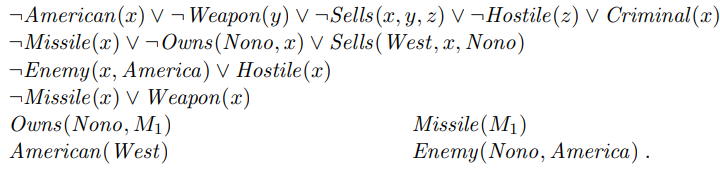
\includegraphics[]{images/crime-cnf.png}
    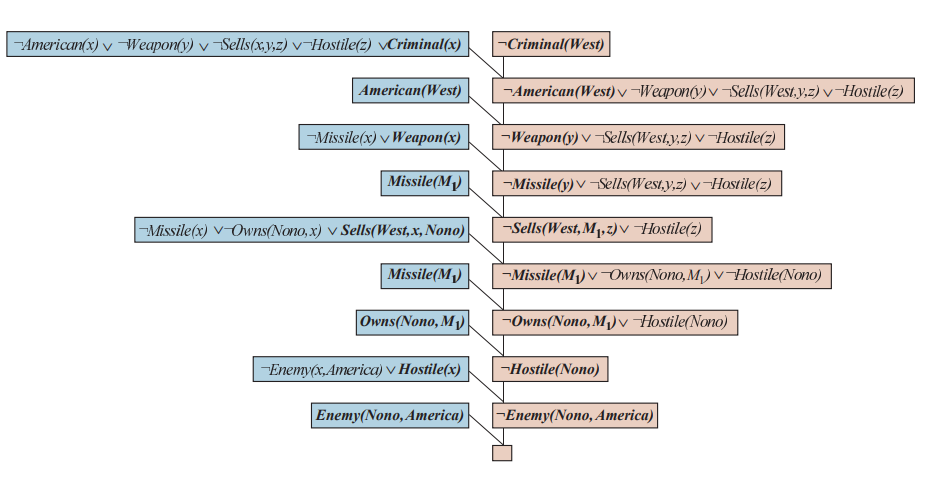
\includegraphics[]{images/resolution-crime-fol.png}
\end{center}
The resolution proof is shown in the figure above. Notice the structure: single “spine” beginning with the goal clause, resolving against clauses from the knowledge base until the empty clause is generated. This is characteristic
of resolution on Horn clause knowledge bases. In fact, the clauses along the main spine correspond exactly to the consecutive values of the goals variable in the backward-chaining algorithm.\\\\
Our second example makes use of Skolemization and involves clauses that are not definite clauses. This results in a somewhat more complex proof structure. In English, the problem is as follows:
\begin{center}
    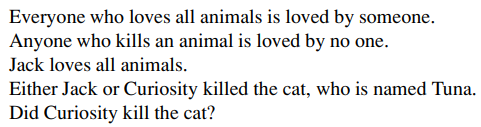
\includegraphics[]{images/resolution-fol-proof.png}
\end{center}
First, we express the original sentences, some background knowledge, and the negated goal G in first-order logic:
\begin{center}
    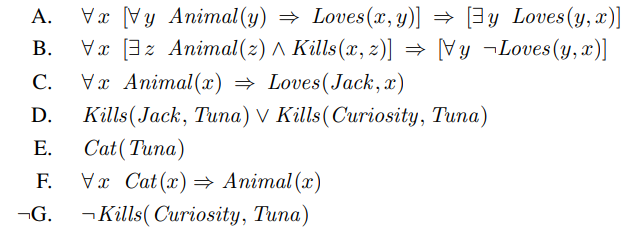
\includegraphics[]{images/kb-res-proof.png}
\end{center}
Now we apply the conversion procedure to convert each sentence to CNF:
\begin{center}
    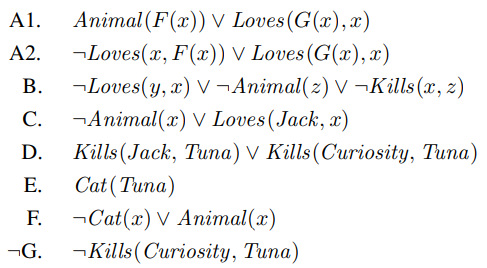
\includegraphics[]{images/kb-cnf-re-prrof.png}
\end{center}
The resolution proof that Curiosity killed the cat is given in the figure below:
\begin{center}
    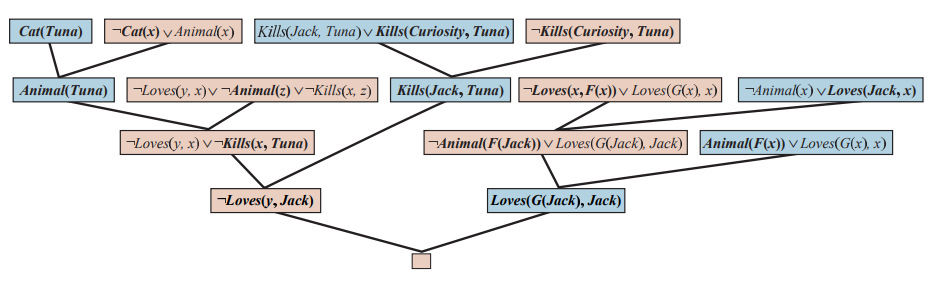
\includegraphics[]{images/res-proof-tree.png}
\end{center}
The proof answers the question “Did Curiosity kill the cat?” but often we want to pose more general questions, such as “Who killed the cat?”. Then, the goal is $\exists w \, Kills(w, Tuna)$, which, when negated, becomes $\neg Kills(w, Tuna)$ in CNF. Repeating the proof with the new negated goal, we obtain a similar proof tree, but with the substitution {w/Curiosity} in one of the steps. Unfortunately, resolution can produce \textbf{nonconstructive proofs} for existential goals. For example, $\neg Kills(w, Tuna)$ resolves with $Kills(Jack, Tuna) \lor Kills(Curiosity, Tuna)$ to give $Kills(Jack, Tuna)$, which resolves again with $\neg Kills(w, Tuna)$ to yield the empty clause. Notice that $w$ has two different bindings in this proof; resolution is telling us that, yes, someone killed Tuna, either Jack or Curiosity. This is no great surprise!
\begin{center}
    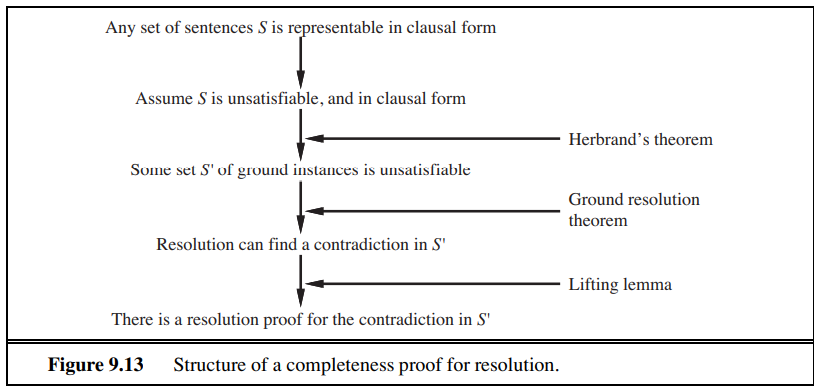
\includegraphics[]{images/res-completeness-fol.png}
\end{center}

\section{Resolution strategies}
We know that repeated applications of the resolution inference rule will eventually find a proof if one exists. In this subsection, we examine strategies that help find proofs efficiently.
\begin{itemize}
    \item \textbf{Unit preference/clause}: prefers to do resolutions where one of the sentences is a single literal.  The idea behind the strategy is that we are trying to produce an empty clause, so it might be a good idea to prefer inferences that produce shorter clauses.

    \item \textbf{Unit resolution:} is a restricted form of resolution in which every resolution step \textbf{must} involve a unit clause. Unit resolution is incomplete in general, but complete for Horn clauses. Unit resolution proofs on Horn clauses resemble forward chaining.

    \item \textbf{Set of support:} every resolution step involve at least one element of a special set of clauses (the set of support); the resolvent is then added into the set of support. Incomplete if the wrong set of support is chosen.

    \item \textbf{Input resolution:} In this strategy, every resolution combines one of the input sentences (from the KB or the query) with some other sentence. Complete for knowledge bases that are in Horn form, but incomplete in the general case. Input resolution has the characteristic shape of a single “spine” with single sentences combining onto the spine. The \textbf{linear resolution} strategy is a slight generalization that allows $P$ and $Q$ to be resolved together either if $P$ is in the original KB or if $P$ is an ancestor of $Q$ in the proof tree. Linear resolution is complete.

    \item \textbf{Subsumption:} eliminates all sentences that are subsumed by (that is, more specific than) an existing sentence in the KB. For example, if $P(x)$ is in the KB, then there is no sense in adding $P(A)$ and even less sense in adding $P(A) \lor Q(B)$. Subsumption helps keep the KB small and thus helps keep the search space small.

\end{itemize}

\chapter{Lec 14 - Higher-order functions for trees III}

\section{Trees type definition}
Until now we used binary trees that support data only in the leaves. Let's change the type definition in order to support information attached to nodes. We can do this in many different ways:
\begin{lstlisting}[style = FSharpStyle]
    type 'a tree =
        | Node of 'a * 'a tree * 'a tree
        | Leaf of 'a
\end{lstlisting}
In this case, a node is composed by an element of type 'a (which is the information attached to it) and the two sub-trees. However, with this definition we wouldn't be able to represent dead branches. In fact, each node must always have two sub-trees that can be either another node or a leaf.
\begin{lstlisting}[style = FSharpStyle]
    type 'a tree =
        | Node of 'a * 'a tree * 'a tree
        | Leaf of 'a option
\end{lstlisting}
With this implementation we can represent a dead branch defining a Leaf of None, but we could even define nodes with two empty leaves. So, this definition allows the programmer to write things that are not in their most simplified form.\newline\newline
In order to prevent this, we can do the following:
\begin{lstlisting}[style = FSharpStyle]
    type 'a tree =
        | Node of 'a * 'a tree option * 'a tree option
\end{lstlisting}
Now the \textbf{Node} data-constructor is a triple composed by:
\begin{itemize}
    \item An element of type 'a (information in the node)
    \item Two 'a tree option elements which represent the left and right sub-trees
\end{itemize}
When both the sub-trees are None, we are representing a leaf.\newline\newline
Let's write in F\# the following tree using this definition:\newline
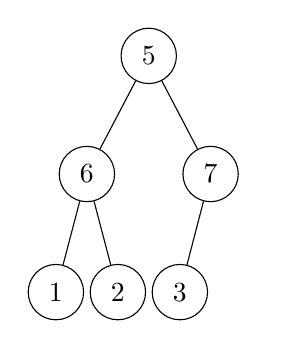
\begin{tikzpicture}
    \Tree
    [.5  
        [.6
            \edge[]; {1}
            \edge[]; {2}
        ]
        [.7
            \edge[]; {3}
            \edge[blank]; \node[blank]{};
        ]
    ]
\end{tikzpicture}\newline
\begin{lstlisting}[style = FSharpStyle]
    let Leaf x = Some(Node(x, None, None))
    let tree = Node(5,
                Some(Node(6, Leaf 1, Leaf 2)),
                Some(Node(7, Leaf 3, None)))
\end{lstlisting}
Note that \textbf{Leaf x} is a function, not a data-constructor. It is just a shorter way to define leaves. The difference between functions and data-constructors is that functions can be used to \textbf{create}, but not for deconstructing (they can't be used to pattern-match).\newline\newline
We can write trees even in a shorter form by defining the following function:
\begin{lstlisting}[style = FSharpStyle]
    let SNode (x, t1, t2) = Some (Node (x, t1, t2))
    let tree = Node (5, 
               SNode (6, Leaf 1, Leaf 2), 
               SNode (7, Leaf 3, None)
               )
\end{lstlisting}
How can we pattern-match this type definition ? We have to specify all possible combinations of node types.
\begin{lstlisting}[style = FSharpStyle]
    let rec pretty_tree t = 
        match t with
        | Node(x, None, None) -> sprintf "(. %O .)" x
        | Node(x, Some l, Some r) -> sprintf "(%s %O %s)" (pretty_tree l) x (pretty_tree r)
        | Node(x, Some l, None) -> sprintf "(%s %O %s)" (pretty_tree l) x "."
        | Node (x, None, Some r) -> sprintf "(%s %O %s)" "." x (pretty_tree r)
        
    let st = pretty_tree tree

    // val st : string = "(((. 1 .) 6 (. 2 .)) 5 ((. 3 .) 7 .))"
\end{lstlisting}
The function above is a \textbf{pretty\_print} function for trees, which is a function that produces a string that represents the given tree. Instead of specify all the possibilities in the pattern-match, we can simplify things by defining an additional function. 
\begin{lstlisting}[style = FSharpStyle]
    let pretty_opt f o = 
        match o with 
        | None -> "."
        | Some x -> f x

    let rec pretty_tree t =
        match t with
        | Node (x, lo, ro) -> 
            let l = pretty_opt pretty_tree lo
            let r = pretty_opt pretty_tree ro
            sprintf "(%s %O %s)"  l x r
    
    let st = pretty_tree tree

    // val st : string = "(((. 1 .) 6 (. 2 .)) 5 ((. 3 .) 7 .))"
\end{lstlisting}
\section{Record types}
In F\# we can define the so called \textbf{record types} using the following syntax:
\begin{lstlisting}[style = FSharpStyle]
    type 'a tree = {data : 'a;
                     left : 'a tree option;
                     right : 'a tree option}
\end{lstlisting}
Records are series of \textit{Label : type} separated by a semicolon.


\chapter{Lec 15-16 Part I - Type inference in F\#}

\section{Simple type inference algorithm}
The type inference algorithm automatically understands the type of an expression in a formal language. Let's consider the following F\# functions with their respective types:
\begin{lstlisting}[style=FSharpStyle]
    let f a b c = if a then b c else a
    //val f : a:bool -> b:('a -> bool) -> c:'a -> bool
    
    let g x y z = (x, y, z)
    //val g : x:'a -> y:'b -> z:'c -> 'a * 'b * 'c

    let h x y z = z y x
    //val h : x:'a -> y:'b -> z:('b -> 'a -> 'c) -> 'c
\end{lstlisting}
A simple type inference high-level algorithm could be the following:
\begin{enumerate}
    \item Bind unknown types to the parameters ('a, 'b, 'c, ...). We will call these unknown types \textbf{type variables}.
    \item \textbf{Substitute} each type variable with a concrete type (if possible) according to what is written in the body of the function. Once a concrete type (int, float, bool, ...) is fixed, it doesn't change anymore. If we need to substitute more that one concrete type it means there is an error in the function.
\end{enumerate}
For example, if we change the definition of f as follows:
\begin{lstlisting}[style=FSharpStyle]
    let f a b c = if a then b c else a+1
\end{lstlisting}
it produces an error because \textit{a} was inferred as bool but is used as an int in the \textit{else} branch of the \textit{if-then-else} statement.
\begin{lstlisting}[style=FSharpStyle]
    let f a b c = if a+1 > 3 then b c else a
\end{lstlisting}
Since the \textit{if-then-else} statement must return the same type in both the branches, the type of the new definition of f is:
\begin{lstlisting}[style=FSharpStyle]
    int -> ('a -> int) -> 'a -> int
\end{lstlisting}
\begin{itemize}
    \item \textit{a} has type int
    \item Also the function \textit{b} produces an int
\end{itemize}
In the body of the function g there are no \textbf{constraints} that permit the type inference to substitute any concrete type, so it will remain a polymorphic function with respect to all the parameters.\newline\newline
Let's insert a constraint in the body of the function g.
\begin{lstlisting}[style=FSharpStyle]
    let g x y z = (x-1, y, z)
\end{lstlisting}
With this change, the compiler understands that \textit{x} must be an integer (due to the constraint x-1), while y and z remain unknown (polymorphic). Polymorphism arises from not knowing any constraint on a type. \newline\newline
Now we can define a more detailed pipeline of the type inference algorithm:
\begin{enumerate}
    \item Bind unknown types to parameters (type variables)
    \item Create a list of constraints according to the body of the function
    \item Check the list of constraints:
           \begin{enumerate}
               \item Eliminate trivial constraints
               \item If two or more constraints for the same type variable are found, produce an error
           \end{enumerate} 
    \item Substitute to each type variable a concrete type, according to the constraints list, to find the final type.    
\end{enumerate}
Let's make an example:
\begin{lstlisting}[style=FSharpStyle]
    let j x = if x then x else x
\end{lstlisting}
\begin{enumerate}
    \item We start by binding unknown types:
    \begin{lstlisting}[style=FSharpStyle]
        j: 'a -> 'b
    \end{lstlisting}
    \item The \textit{if-then-else} statement requires two constraints:
        \begin{itemize}
            \item The guard of the \textit{if} must be a bool
            \item The two branches must produce the same type
        \end{itemize}
    So the list of constraints becomes:
    \begin{lstlisting}[style=FSharpStyle]
        'a -> bool
        'a -> 'a
        'b -> 'a
    \end{lstlisting}
    By eliminating trivial constraints the list becomes:
    \begin{lstlisting}[style=FSharpStyle]
        'a -> bool
        'b -> 'a
    \end{lstlisting}
    Then, we simplify the constraints list:
    \begin{lstlisting}[style=FSharpStyle]
        'a -> bool
        'b -> bool
    \end{lstlisting}
    \item Since there are not multiple constraints for the same type variable, we can perform the substitution. The type of j becomes:
    \begin{lstlisting}[style=FSharpStyle]
        j: bool -> bool
    \end{lstlisting}
    The substitution can be seen as a function from type variables to types:
    \[ \Theta: \alpha \rightarrow \tau\]
\end{enumerate}
Note that if we had written the following expression:
\begin{lstlisting}[style=FSharpStyle]
    let j x = if x then x else 2
\end{lstlisting}
the constraints list would have been:
\begin{lstlisting}
    'a -> bool
    'a -> int
    'b -> int
\end{lstlisting}
So, the type inference algorithm would have produced an error since there are multiple constraints for the type variable 'a.


\chapter{Lec 15-16 Part II - Type checking rule}

\section{Inference logic rule}
\[
    \infer{\Gamma \vdash \lambda x.e : \tau_{1} \rightarrow \tau_{2}}{\Gamma, (x:\tau_{1}) \vdash e:\tau_{2}}\]
The formula above, in the world of logic, is called \textbf{inference logic rule}. Basically, it is an implication from "\textit{up}" to "\textit{down}". It means that the formula above the horizontal line implies the formula below.\newline\newline
In order to understand this rule, we need to define its terms.
\subsection{Expressions}
\label{expr}
$e$ is an \textbf{expression} defined through a \textbf{BNF} grammar:
\begin{grammar}
    <e> ::= <x>
    \alt <λx.e> 
    \alt <e e>
    \alt <Let x = e in e>
\end{grammar}
An expression $e$ can either be:
\begin{itemize}
    \item A variable name
    \item A lambda
    \item An application
    \item A let binding
\end{itemize}
Let's consider the following expression in F\#:
\begin{lstlisting}[style=FSharpStyle]
    let m = (1+2+3) 4
\end{lstlisting}
The right part of the let binding is correct from the point of view of the syntax (it's an application), but is wrong from the point of view of types. So, a compiler can be seen as a pipeline:
\begin{enumerate}
    \item First checks the syntax
    \item Then understands types (type inference)
\end{enumerate}
    
\subsection{Types}
A type $\tau$ is defined as a syntactic entity through a BNF grammar:
\begin{grammar}
    <τ> ::= <c>
    \alt <τ ⟶ τ >
    \alt α
\end{grammar}
Where $c$ is a constant type name (e.g. int, float, bool, ...) and $\alpha$ is a \textbf{generic} type variable.

\subsection{The environment $\Gamma$}
$\Gamma$ is the environment (scope) and is defined as follows:
\begin{grammar}
    <Γ> ::= Ø
    \alt <Γ,(x : τ) >
\end{grammar}
Let's consider the following F\# code:
\begin{lstlisting}[style=FSharpStyle]
    let f a b c = if a then b c else a

    let myfun x y=
        let f z = f x y x
        f 3
\end{lstlisting}
Note that when we bind \textit{f} inside \textit{myfun}, since it is not specified the \textbf{rec} keyword, we are referring to the definition of \textit{f} written above \textit{myfun}. So, in order to analyze the type of the nested function \textit{f} defined inside \textit{myfun}, the compiler must have memorized the type of the function \textit{f} defined above \textit{myfun}. In F\# the let binding adds an entry to the scope, but how can we represent this information ? \newline\newline
The simplest way for representing the scope is a sequence of pairs, where each pair is composed by an identifier and its type. $\Gamma$ can be seen as a function from the set of identifiers $X$ to types:
\[\Gamma: X \rightarrow \tau\]
\subsection{Understanding the formula}
Let's go back to the logic rule mentioned before:
\[
    \infer{\Gamma \vdash \lambda x.e : \tau_{1} \rightarrow \tau_{2}}{\Gamma, (x:\tau_{1}) \vdash e:\tau_{2}}\]
\begin{itemize}
    \item $\vdash$ means "\textit{deduce}"
    \item : means "\textit{has type}"
\end{itemize}
so, a literal translation of $\Gamma \vdash e : \tau$ would be: "\textit{In a scope $\Gamma$, we deduce that the expression $e$ has type $\tau$}".\newline\newline
The meaning of the whole formula is the following: Given a lambda $\lambda x.e$ in an environment $\Gamma$, if we extend the scope $\Gamma$ by binding to the parameter $x$ the type $\tau_{1}$ and we deduce that the body $e$ has type $\tau_{2}$, then the lambda must have type $\tau_{1} \rightarrow \tau_{2}$.  Basically, it says that the domain of the lambda is the type of the parameter and the codomain is the type of the body.\newline\newline
This is a \textbf{type checking} rule because it says what must be true for an expression in order to be valid from the point of view of types, but it doesn't show how to infer types. Type inference shows how to automatically understands types, rather than just assuming them.\newline\newline
Let's make an example in F\#:
\begin{lstlisting}[style=FSharpStyle]
    let r  = fun x -> x 23
\end{lstlisting}
The right part of the let binding is a lambda that has an application as body. The type inference understands that:
\begin{itemize}
    \item the parameter $x$ has type int $\rightarrow$ 'a
    \item the expression $e$, that is an application, has type 'a
\end{itemize}
Then, by applying the type checking rule, the whole lambda must have type (int $\rightarrow$ 'a) $\rightarrow$ 'a\newline\newline
It is useful to express the type checking algorithm through a series of logical implications. This is because we want to describe the algorithm in such a way that we can derive some mathematical properties. The most important property that we can derive from this definition is \textbf{soundness}.\newline\newline
Soundness means that given a program, if the types are correct then the program works (in the sense that run without crashing). Note that, in functional languages, every program is an expression made of multiple let bindings.
\subsection{Type checking rule for the other expression terms}
We defined the type-checking rule only for the lambda-term of expressions. Let's write the same rule with respect to application, variable name and let binding terms (according to the definition of expression we gave in section \ref{expr}). 
\begin{itemize}
    \item \textbf{Variable name:} 
    \[ \infer{\Gamma \vdash x : \tau}{ \begin{gathered} x \in domain(\Gamma)\\ \Gamma(x) = \tau \end{gathered}} \]
    A variable $x$ has type $\tau$ in the scope $\Gamma$ if it is defined in the scope and if $\Gamma$ applied to $x$ produces $\tau$ ($\Gamma$ is a function as we said previously).
    \item \textbf{Application:} 
    \[ \infer{\Gamma \vdash e_{1} \, e_{2} : \tau_{2}}{\begin{gathered} \Gamma \vdash e_{1} : \tau_{1} \rightarrow \tau_{2} \\ \Gamma \vdash e_{2} : \tau{1} \end{gathered}}\]

    \item \textbf{Let binding:}
    \[ \infer{\Gamma \vdash let \, x = e_{1} \, in \, e_{2} : \tau_{2}}{\begin{gathered}
        \Gamma \vdash e_{1} : \tau_{1}\\
        \Gamma, (x:\tau_{1}) \vdash e_{2}:\tau_{2}
    \end{gathered}}\]
    Let's make an example in F\#:
    \begin{lstlisting}[style=FSharpStyle]
        let a=3 in let b = true in a
    \end{lstlisting}
    In this example $e_{1} = 3$ and $e_{2} =$ \textit{let b = true in a }. The rule that type checks the binding \textit{let a = 3} is $\Gamma \vdash e_{1}:\tau_{1}$. In our example $\tau_{1}=int \rightarrow e_{1}:int$. Then, we bind \textit{(a:int)} and we add this information to the original scope. By recursively repeating the type-checking for $e_{2}$ in the extended scope, we'll eventually have the environment $\Gamma$ composed by: $\{(a:int), (b:int)\}$ and the variable \textit{a}
    will be type-checked following the rule mentioned before. 
\end{itemize}


\chapter{Lec 16 - Graph Neural Networks}

\section{Introduction}
Traditional ML approaches have been developed assuming data to be encoded into feature vectors; however, many important real-world applications generate data that are naturally represented by more complex structures, such as graphs. Graphs are particularly suited to
represent the relations (arcs) between the components (nodes) constituting an entity. For instance, in social network data, single data “points” (i.e., users) are closely inter-related.\newline\newline
A graph $G = (V, E)$ can be represented using the so called \textbf{adjacency matrix}. A $n \times n$ matrix $A$ such that $A[i,j] = 1$ if $edge(i,j) \in E$, 0 otherwise.\newline\newline
    \textbf{Example:}\newline\newline
    \begin{center}
        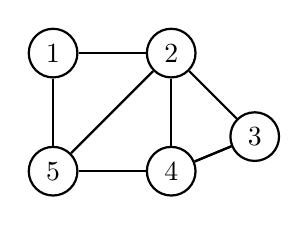
\begin{tikzpicture}[node distance={15mm}, thick, main/.style = {draw, circle}] 
            \node[main] (1) {$1$}; 
            \node[main] (2) [right of=1] {$2$}; 
            \node[main] (3) [below right of=2] {$3$}; 
            \node[main] (4) [below of=2] {$4$}; 
            \node[main] (5) [below of=1] {$5$}; 
            \draw (1) -- (2); 
            \draw (1) -- (5); 
            \draw (2) -- (5);
            \draw (2) -- (4);
            \draw (5) -- (4);
            \draw (3) -- (4); 
            \draw (5) -- (4);
            \draw (4) -- (3);
            \draw (2) -- (3);
        \end{tikzpicture}
    \end{center}
    The Adjacency matrix of the graph above is the following:
    \[\begin{bmatrix}
        0 & 1 & 0 & 0 & 1 \\
        1 & 0 & 1 & 1 & 1 \\
        0 & 1 & 0 & 1 & 0 \\
        0 & 1 & 1 & 0 & 1 \\
        1 & 1 & 0 & 1 & 0
    \end{bmatrix}\]
In undirected graphs this matrix is \textbf{symmetric}, while in directed graphs it is \textbf{asymmetric}. In case of a weighted graph, each cell of the matrix has either the value of the edge weight $w$ or $-$. Each node and edge is represented by a feature vector:
\begin{center}
    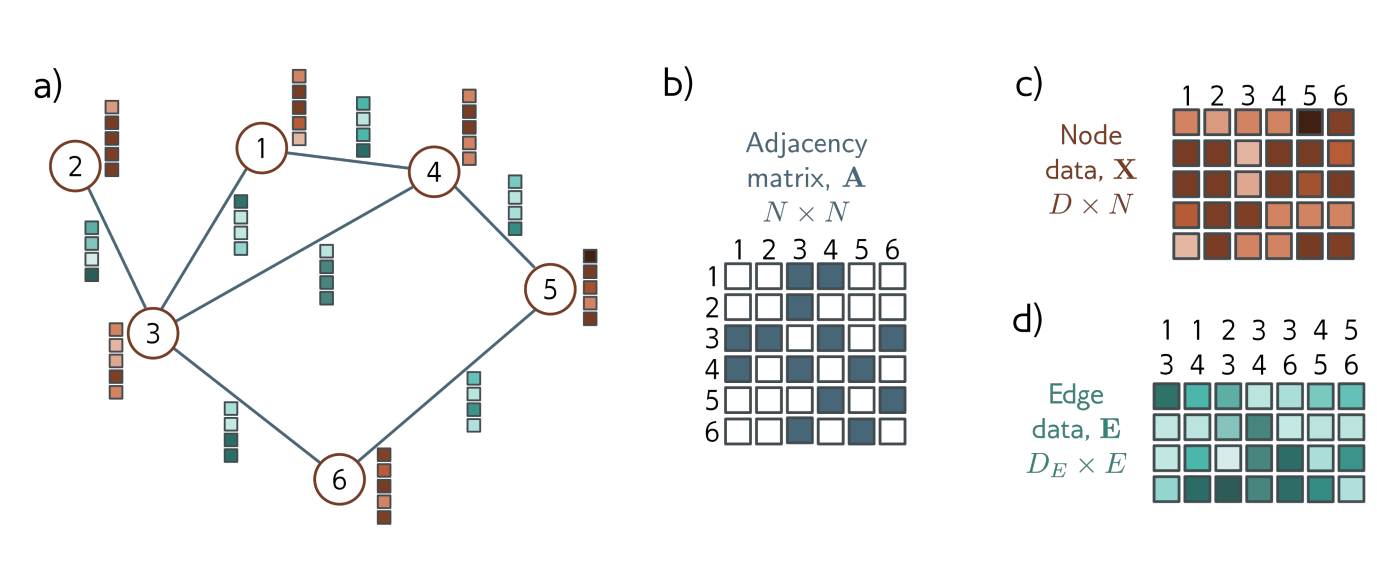
\includegraphics[scale=0.5]{images/graphs.png}
\end{center}
The position $(m,n)$, of the adjacency matrix contains the number of walks of length one from node $m$ to node $n$. Position $(m,n)$ of the \textbf{squared} adjacency matrix $A^2$ contains the number of walks of length two from node $m$ to node $n$.\newline\newline
The main problem settings that can arise when dealing with structured data are the following:
\begin{itemize}
    \item Predictions over \textbf{nodes} in a network: In this setting, the dataset is composed of a single (possibly disconnected) large graph. Each example is a node in the graph, and the learning tasks are defined as predictions over the nodes. Given an unseen node $u$, the task is to predict the correct target $y_u$. An example in this setting is the prediction of properties of a social network user based on his or her connections.

    \item Predictions over \textbf{graphs}: In this case, each example is composed of a whole graph, and the learning tasks are predictions of properties of the whole graphs. An example is the prediction of toxicity in humans of chemical compounds represented by their molecular graph.

    \item Link-prediction tasks: the model predicts whether or not there should be an edge between nodes. 
\end{itemize}

\section{Learning on graphs is difficult}
Let $\textbf{X}$ be the matrix in which the feature vectors of each node are stored. We can observe that node indexing in graphs is arbitrary. This means that, differently from images, permuting the node indices results in a permutation of the columns of $\textbf{X}$ and a permutation of both the rows and columns of $A$. However, the underlying graph is unchanged. This property is called Permutation Invariance. More formally, given a permutation matrix $\textbf{P}$, we get a different representation of the same graph:
\[\begin{split}
    \textbf{X}' & = \textbf{XP}\\
    \textbf{A}' & = \textbf{P}^T \textbf{AP}
\end{split}
\]
This property can give the intuition about why learning on graphs is difficult. In fact, determining if two graphs are equal (graphs isomorphism) is a problem for which are not known polynomial-time algorithms. Furthermore, sub-graph isomorphism, which is the problem of determining if a graph is a sub-graph of another graph, is NP-Complete. These problems affect machine learning because a model should be able to predict the same output for isomorphic graphs (which can be represented in different ways). Furthermore, the model we design should capture the similarity between two graphs (sub-graph isomorphism).\newline\newline
In general, the main problems we face when learning on graphs are the following:
\begin{enumerate}
    \item Same graph can be represented in different ways;
    \item How to recognize that a given graph $G_2$ is a sub-graph of $G_1$
    \item How to represent graphs of different sizes (i.e., different number of nodes) into fixed-size vectors without loosing expressiveness ?

    \item How to avoid explosion in the number of parameters with the size of the graphs?
    
\end{enumerate}
Problem 3 is commonly faced by using recursive models that exploit a
causal state space [Sperduti \& Starita., TNN 1997], while Problem 4  is commonly faced by exploiting shared parameters.\newline\newline
Regarding Problems 1 and 2, a sound and meaningful representation for graphs can be achieved by using a neural network with \textbf{convolution operator}, defined on graphs.

\section{Graph Neural Networks - General Idea}
A Graph Neural Network (GNN) receives in input a graph (adj. matrix and node representations. for simplicity) and passes it through a series of $k$ layers. Each layer computes a hidden representation for each node, with the last layer computing the final nodes' embeddings $\textbf{H}_k$. Similarly to CNNs, each node representation includes information about the node and its context within the graph.
\begin{itemize}
    \item For \textbf{node-level tasks}, the output is computed from $\textbf{H}_k$;

    \item For \textbf{graph-level tasks}, the nodes' embeddings are combined (e.g., by averaging), and the resulting vector is mapped via a linear transformation or neural network to a fixed-size vector from which the classification/regression task is performed.

    \item For \textbf{link-prediction tasks}, the embeddings of the two endpoint nodes must be mapped to a single number representing the probability that the edge is present (e.g. dot product of the nodes' embeddings and pass the result through a sigmoid function to create a probability).
 
\end{itemize}
\begin{center}
    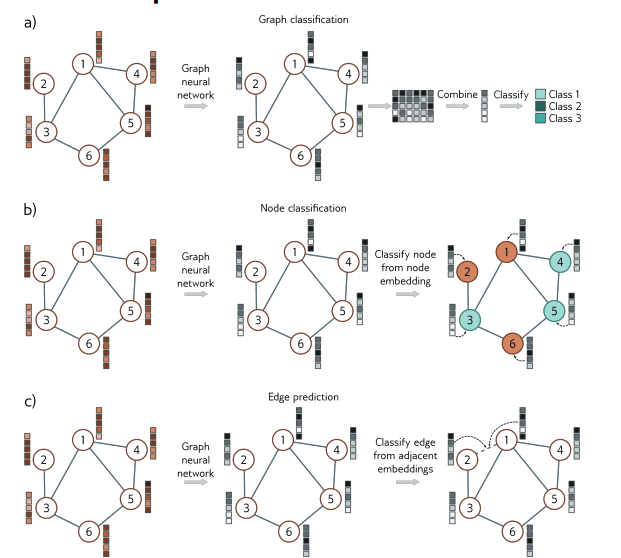
\includegraphics[]{images/gnn.png}
\end{center}

\section{Graph Convolution}
The general idea of graph convolution starts from a parallel between graphs and images. GNNs implement convolution in a similar way how CNNs do, that is, learning the features by inspecting neighboring nodes. GNNs generalize the definition of convolution for non-regular structured data.

\subsection{NN4G by Micheli}
\textbf{NN4G} is an architecture based on a graph convolution that is defined as:
\begin{center}
    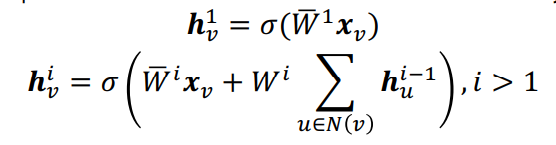
\includegraphics[scale=0.6]{images/nn4g.png}
\end{center}
where: 
\begin{itemize}
    \item $\sigma$ is a nonlinear activation function applied element-wise.
    \item $N(v)$ represent the neighborhood of node $v$.
    \item $\textbf{W}^i$ is a weights' matrix;
    \item $\textbf{x}_u$ is the feature vector of node $u$.
\end{itemize}
Actually, this is a simplified notation, since the original one uses skip connections (see GNN book chapter).
\begin{center}
    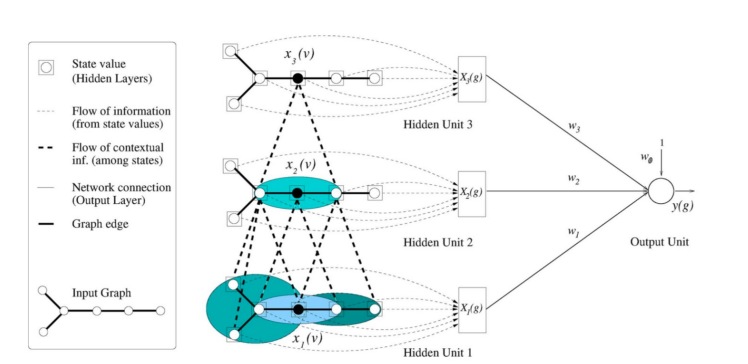
\includegraphics[]{images/nn4g-2.png}
\end{center}
Note that:
\begin{itemize}
    \item The first layer ($i = 1$), which has no previous layers, computes the nodes' representations only on the basis of each vertex feature vector.

    \item Each convolution performed on the $i$-th hidden units, with $i > 1$, takes as input the neighbors' representations of the previous layer. Basically, it merges the representations of each node with those of its neighbors:

    \item $X_1(g), X_2(g), X_3(g)$ are scalar values computed by aggregating the representations $\textbf{x}_i(g)$ for each unit $i$.
    In particular they are defined as:
    \[X_i(g) = \frac{1}{k}\sum_{v \in Vert(g)}x_i(v)\]
    if $k = 1$, this corresponds to a sum. Basically, we compute a representation per-graph per-layer. Then, this 3 representations are parametrized by the weights $w_1, w_2, w_3$ and used to compute the output for the whole graph (graph-level task).
\end{itemize}
The convolutional operation presented above can be defined in a compact way using matrix multiplications:
\begin{center}
    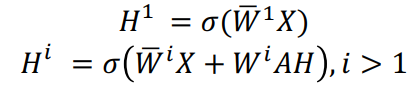
\includegraphics[scale=0.6]{images/matrix-gcn.png}
\end{center}
where $\textbf{A}$ is the adjacency matrix. Exploiting matrix multiplications makes the computation really fast. Furthermore, note that, as for images, the receptive field of the layers increases as we stack more layers.\newline\newline
Note also that, since with the convolution operator we are merging neighboring nodes' representations, isomorphic graphs in which the order of the nodes is changed will have the same nodes' representations.

\subsection{Graph Fourier Transform}
The operation described above is graph convolution, but how it is derived? Defining the formal convolution operator on graph is difficult.\newline\newline
Let $x: V \rightarrow \mathbb{R}$ be a signal on the nodes $V$ of the graph $G$, i.e., a function that associates a real value with each node of $V$. We can represent every signal as a vector $\textbf{x} \in \mathbb{R}^n$, which from now on we will refer to as signal. In order to set up a convolutional network on $G$, we need the notion of convolution between a signal $\textbf{x}$ and a filter signal $\textbf{f}$.\newline\newline
The key idea is to use a Fourier transform. In the frequency domain, thanks to the \textbf{Convolution Theorem}, the (undefined) convolution of two signals becomes the (well-defined) component-wise product of their transforms. So, if we knew how to compute the Fourier transform of a function defined on a graph, we could define the convolution operator.\newline\newline
The Convolution Theorem states that convolution in one domain (time, space) corresponds to pointwise multiplication in frequency domain.\newline\newline
The \textbf{graph Fourier transform} is defined starting from the (normalized) Laplacian matrix of the graph, which is defined as:
\[L = I_n - D^{-\frac{1}{2}} A D^{-\frac{1}{2}}\]
where:
\begin{itemize}
    \item $I_n$ is the identity matrix;
    \item $A$ is the adjacency matrix;
    \item $D$ is the degree matrix, that is, the \textbf{diagonal} matrix containing the number of edges attached to each vertex;
\end{itemize}
Then, we can compute the eigendecomposition of $L$ (which is always possible):
\[L = U \Lambda U^T\]
where $\Lambda = diag([\lambda_0, ..., \lambda_{n-1}])$ and $U$ is the Fourier basis of the graph.\newline\newline
Finally, Given a spatial signal $\textbf{x}$:
\begin{itemize}
    \item $\hat{\textbf{x}} = U^T\textbf{x}$ is its graph Fourier Transform

    \item $\textbf{x} = U \hat{\textbf{x}}$ is the inverse Fourier transform
\end{itemize}
Therefore, convolution between a parametric filter and a signal can be defined as:
\[y = \textbf{f}_\theta *_G \textbf{x} = U\left( (U^T\textbf{f}_\theta) \odot (U^T \textbf{x})\right)\]
It can be proved that this operator corresponds to the one used for NN4G presented previously (see slides for more details).

\section{Aggregation Layer for graph classification}
With Graph Convolution we have a representation for each graph node. How can we map node representations to a graph-level representation? There are some simple solutions, like the sum or the average of nodes' representations as we saw previously, or we can rely on more complex alternatives: Universal readout.


\section{Graph Recurrent Neural Networks}
Scarselli et al. proposed a network architecture where, instead of stacking multiple layers, a single recurrent layer is adopted:
\[\textbf{h}_v^{t+1} = \sum_{u \in N(v)}f(\textbf{h}_u^t, \textbf{x}_v, \textbf{x}_u)\]
where $f$ is a function (e.g. neural network) with shared parameters across all the nodes and all the time steps. The recurrent system is defined as a contraction mapping, and thus it is guaranteed to converge to a fixed point $\textbf{h*}$.

\subsection{Gated Graph Neural Networks}
The idea is to remove the constraint for the recurrent system to be a contraction mapping, and implement this idea by adopting recurrent
neural networks to define the recurrence. Specifically, the gated recurrent unit (GRU) is adopted. The recurrent convolution operator is defined as follows:
\begin{center}
    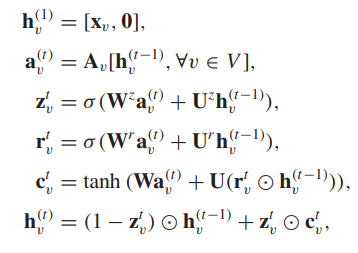
\includegraphics[scale=0.8]{images/gated-gnn.png}
\end{center}
where $\textbf{A}_v$ is row $v$ of the adjacency matrix $\textbf{A}$.




\end{document}
